\section{Verzamelingen}

\begin{answer} % 4.1
In het onderstaande plaatje is $U$ het universum, en zijn $A$ en $B$ verzamelingen. Teken dit plaatje een aantal malen over, en geef door kleur/arcering aan:

\begin{enumerate}[label=\textbf{\alph*.}]

    % a:
    \item $A\Delta B$ (symmetrisch verschil tussen $A$ en $B$ \\
    antwoord: \\
    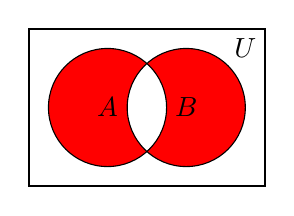
\begin{tikzpicture}[scale=.5]
    
    \def\firstcircle{(0,0) circle (1.5cm)}
    \def\secondcircle{(0:2cm) circle (1.5cm)}
    \def\universe{(-2,-2) rectangle (4,2)}

    %Color stuff:
    \begin{scope}[even odd rule]
        \clip \secondcircle (0,0) \universe;
        \fill[red] \firstcircle;
    \end{scope}
    %Color more stuff:
    \begin{scope}[even odd rule]
        \clip \firstcircle (0,0) \universe;
        \fill[red] \secondcircle;
    \end{scope}
    
    %draw circles:
    \draw \firstcircle node {$A$};
    \draw \secondcircle node {$B$};
    
    %draw universe:
    \draw[thick] \universe;
    \node at (3.5,1.5) {$U$};

    \end{tikzpicture}
    
    % b:
    \item $A^c\Delta B^c$ \\
    antwoord:\\
    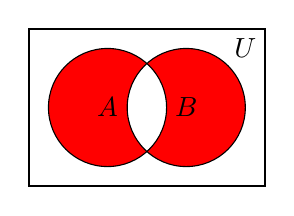
\begin{tikzpicture}[scale=.5]
    
    \def\firstcircle{(0,0) circle (1.5cm)}
    \def\secondcircle{(0:2cm) circle (1.5cm)}
    \def\universe{(-2,-2) rectangle (4,2)}

    %Color stuff:
    \begin{scope}[even odd rule]
        \clip \secondcircle (0,0) \universe;
        \fill[red] \firstcircle;
    \end{scope}
    %Color more stuff:
    \begin{scope}[even odd rule]
        \clip \firstcircle (0,0) \universe;
        \fill[red] \secondcircle;
    \end{scope}
    
    %draw circles:
    \draw \firstcircle node {$A$};
    \draw \secondcircle node {$B$};
    
    %draw universe:
    \draw[thick] \universe;
    \node at (3.5,1.5) {$U$};

    \end{tikzpicture}
    
    %c:
    \item $(A^c-B^c)$\\
    antwoord:\\
    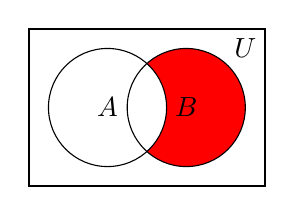
\begin{tikzpicture}[scale=.5]
    
    \def\firstcircle{(0,0) circle (1.5cm)}
    \def\secondcircle{(0:2cm) circle (1.5cm)}
    \def\universe{(-2,-2) rectangle (4,2)}

    %Color stuff:
    \begin{scope}[even odd rule]
        \clip \firstcircle (0,0) \universe;
        \fill[red] \secondcircle;
    \end{scope}
    
    %draw circles:
    \draw \firstcircle node {$A$};
    \draw \secondcircle node {$B$};
    
    %draw universe:
    \draw[thick] \universe;
    \node at (3.5,1.5) {$U$};
    
    \end{tikzpicture}
    % d:
    \item $A-B$\\
    antwoord:\\
    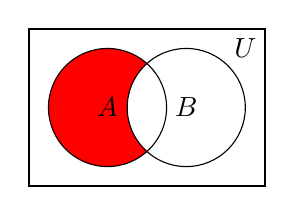
\begin{tikzpicture}[scale=.5]
    
    \def\firstcircle{(0,0) circle (1.5cm)}
    \def\secondcircle{(0:2cm) circle (1.5cm)}
    \def\universe{(-2,-2) rectangle (4,2)}

    \begin{scope}[even odd rule]
        \clip \secondcircle (0,0) \universe;
        \fill[red] \firstcircle;
    \end{scope}
    
    %draw circles:
    \draw \firstcircle node {$A$};
    \draw \secondcircle node {$B$};
    
    %draw universe:
    \draw[thick] \universe;
    \node at (3.5,1.5) {$U$};
    
    \end{tikzpicture}
    
    % e:
    \item $A^c-B$\\
    antwoord:\\
    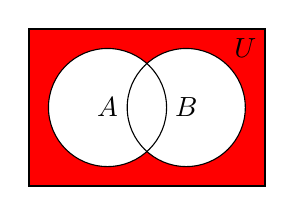
\begin{tikzpicture}[scale=.5]
    
    \def\firstcircle{(0,0) circle (1.5cm)}
    \def\secondcircle{(0:2cm) circle (1.5cm)}
    \def\universe{(-2,-2) rectangle (4,2)}

    %Color stuff:
    \begin{scope}[even odd rule]
        \clip \firstcircle (0,0) \universe;
        \clip \secondcircle (0,0) \universe;
        \fill[red] \universe;
    \end{scope}
    
    %draw circles:
    \draw \firstcircle node {$A$};
    \draw \secondcircle node {$B$};
    
    %draw universe:
    \draw[thick] \universe;
    \node at (3.5,1.5) {$U$};
    
    \end{tikzpicture}
    
    % f:
    \item $(A-B)^c$ \\
    antwoord:\\
    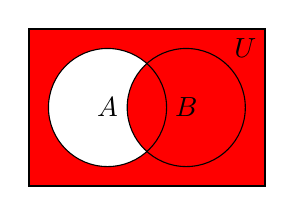
\begin{tikzpicture}[scale=.5]
    
    \def\firstcircle{(0,0) circle (1.5cm)}
    \def\secondcircle{(0:2cm) circle (1.5cm)}
    \def\universe{(-2,-2) rectangle (4,2)}
    
    %Color stuff:
    \begin{scope}[even odd rule]
        \clip \firstcircle (0,0) \universe;
        \clip \secondcircle (0,0) \universe;
        \fill[red] \universe;
    \end{scope}
    
    \fill[red] \secondcircle;
    
    %draw circles:
    \draw \firstcircle node {$A$};
    \draw \secondcircle node {$B$};
    
    %draw universe:
    \draw[thick] \universe;
    \node at (3.5,1.5) {$U$};
    
    \end{tikzpicture}
    
\end{enumerate}
\end{answer}

\begin{answer} % 4.2
Gegeven is dat $A$ de \textit{verzameling is van rode dingen}, en $B$ de \textit{verzameling van grote dingen}, en $x$ een variabele is over een universum $U$ (van objecten). Druk de volgende verzamelingen uit in $A$ en $B$ en de operatoren op verzamelingen:
\begin{enumerate}[label=\textit{\alph*.}]
    \item De verzameling $I$ van objecten die groot zijn als ze rood zijn.\\
    antwoord: \\
    $I = \{ x\;|\;x \in A \rightarrow x \in B\}$ \\
    of: $I = A^c\cup B$
    \item De verzameling $C$ van objecten die rood en groot zijn.\\
    antwoord: \\
    $C = \{x\;|\;x \in A\land x\in B\}$ \\
    of: $C = \{x\in A\;|\;x\in B\}$ \\
    of: $C = A \cap B$
    \item De verzameling $E$ van objecten die rood zijn dan en slechts dan als ze groot zijn.
    antwoord: \\
    $E = \{x\;|\;x\in A \leftrightarrow x\in B\}$ \\
    of: $E = \{x\;|\;(x\in A \land x\not\in B)\lor(x\in B\land x\not\in A)\}$ \\
    of: $E = \{x\;|\;(x\in A\rightarrow x\in B)\land (x\in B\rightarrow x\in A)\}$ \\
    of: $E = (A \cap B)\cup(A^c\cap B^c)$
    \item De verzameling $D$ van objecten die rood of groot zijn.
    antwoord: \\
    $D = \{x | x\in A \lor x\in B\}$\\
    of: $D = A \cup B$
\end{enumerate}
\end{answer}

\begin{answer} % 4.3
Teken de bijbehorende Venn-diagrammen, en bewijs
\begin{enumerate}[label=\textit{\alph*.}]
    % a:
    \item $A-(B-C)=A-(B-(A\cap C))$\\
    antwoord:\\
    venn diagram:\\
    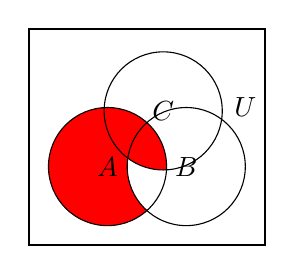
\begin{tikzpicture}[scale=.5]
    
    \def\firstcircle{(0,0) circle (1.5cm)}
    \def\secondcircle{(0:2cm) circle (1.5cm)}
    \def\thirdcircle{(45:2cm) circle (1.5cm)}

    \def\universe{(-2,-2) rectangle (4,3.5)}

    %Color stuff:
    \begin{scope}[even odd rule]
        \clip \thirdcircle;
        %\clip \secondcircle (0,0) \universe;
        \fill[red] \firstcircle;
    \end{scope}
    %colormore stuff:
    \begin{scope}[even odd rule]
        \clip \secondcircle (0,0) \universe;
        %\clip \secondcircle (0,0) \universe;
    \fill[red] \firstcircle;
    \end{scope}
    
    %draw circles:
    \draw \firstcircle node {$A$};
    \draw \secondcircle node {$B$};
    \draw \thirdcircle node {$C$};
    
    %draw universe:
    \draw[thick] \universe;
    \node at (3.5,1.5) {$U$};
    
    \end{tikzpicture}\\

    bewijs: (volledig bewijs hier alleen opgenomen voor volledigheid; bewijzen via andere methode hieronder)\\
    \begin{align}
    A - (B - C) &= x\in A\wedge \neg(x\in B-C)\tag{\text{definitie -}}\\
    &= x\in A\wedge\neg(x\in B\wedge\neg x\in C) \tag{\text{definitie -}}
    \end{align}
    Hernoem nu $x\in A$ naar $p$, $x\in B$ naar $q$ en $x\in C$ naar $r$:
    \begin{align}
    &= p\wedge\neg(q\wedge\neg r)\tag{\text{hernoemen}}\\
    &= p\wedge(\neg q\vee\neg\neg r)\tag{St-2.3.2:10}\\
    &= p\wedge(\neg q\vee r)\tag{St-2.3.2:1}\\
    &=(p\wedge\neg q)\vee(p\wedge r)\tag{St-2.3.2:11}\\
    \end{align}
    Op dit punt is het niet helemaal duidelijk wat je moet doen, maar als je nu van `onderaf' begint en omhoog werkt, dan zie je waar het bewijs sluitend gemaakt kan worden:
    \begin{align}
    &=(p\wedge\neg q)\vee((p\wedge p)\wedge r)\tag{St-2.3.2:1}\\
    &=(p\wedge\neg q)\vee(p\wedge (p\wedge r))\tag{St-2.3.2:6}\\
    &=p\wedge(\neg q)\vee(p\wedge r)\tag{St-2.3.2:11}\\
    &=p\wedge(\neg q\vee\neg\neg (p\wedge r))\tag{St-2.3.2:1}\\
    &=p\wedge\neg(q\wedge\neg(p\wedge r))\tag{St-2.3.2:9}\\
    &=x\in A\wedge\neg(x\in B\wedge\neg (x\in A\wedge x\in C))\tag{\text{hernoemen}}\\
    &=x\in A\wedge\neg(x\in B\wedge\neg (x\in A\cup C))\tag{\text{definitie $\cap$}}\\
    &=x\in A\wedge\neg(x\in B-(A\cap C))\tag{\text{definitie }-}\\
    &=x\in A-(B-(A\cap C)\tag{\text{definitie }-}
    \end{align}
    
    bewijs (eenvoudiger): Gegeven\\
    \begin{tikzpicture}[scale=.5]
    \def\firstcircle{(0,0) circle (1.5cm)}
    \def\secondcircle{(0:2cm) circle (1.5cm)}
    \def\thirdcircle{(45:2cm) circle (1.5cm)}
    
    \def\universe{(-2,-2) rectangle (4,3.5)}
    
    %draw circles:
    \draw \firstcircle;
    \draw \secondcircle;
    \draw \thirdcircle;
	\node at (-1,-1.25) {$A$};
	\node at (3.25, -1.25) {$B$};
	\node at (0.5, 3) {$C$};   
    
    %draw universe:
    \draw[thick] \universe;
    \node at (3.75,3.25) {$U$};
    \begin{scope}[font=\small, color=hured]
	    \node at (-1, 2) {1};
	    \node at (1.5, 2) {2};
    	\node at (.5,1) {3};
	    \node at (1, .5) {4};
	    \node at (2, 1) {5};
	    \node at (-.5, -.5) {6};
	    \node at (1, -.5) {7};
	    \node at (2.5, -.5) {8};
    \end{scope}
    \end{tikzpicture}\\
    $A-(B-C)$: $A$ is 3, 4, 6, 7; $B$ is 4, 5, 7, 8; $C$ is 2, 3, 4, 5; $B-C$ is dan 7, 8 (immers, 4 en 5 zitten ook in $C$); $A-(B-C)$ is dan 3, 4, 6 (want alleen 7 zit in $B-C$).
    
    \noindent
    $A-(B-(A\cap C))$: $A$, $B$ en $C$ zoals hierboven; $A\cap C$ is 3, 4 (beiden is zowel $A$ als $C$); $B-(A\cap C)$ is dan 5, 7, 8 (want alleen 3 in $A\cap C$); $A-(B-(A\cap C))$ is daarmee 3, 4, 6 (want 5 en 8 waren al geen onderdeel van $A$, alleen 7 is onderdeel van $A$ en van $B-(A\cap C)$.
    
    \noindent $A-(B-C)=A-(B-(A\cap C))$ want ze bevatten exact dezelfde venn-diagramonderdelen (semi-formeel bewijs).
    %b:
    \item $(A-B)-C=A-(B\cup C)$\\
    antwoord: \\
    Venn diagram:\\
        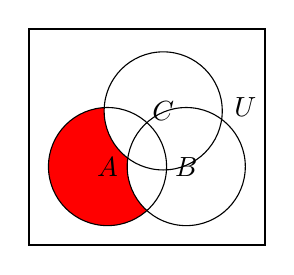
\begin{tikzpicture}[scale=.5]
    
    \def\firstcircle{(0,0) circle (1.5cm)}
    \def\secondcircle{(0:2cm) circle (1.5cm)}
    \def\thirdcircle{(45:2cm) circle (1.5cm)}

    \def\universe{(-2,-2) rectangle (4,3.5)}

    %Color stuff:
    \begin{scope}[even odd rule]
        \clip \thirdcircle (0,0) \universe{};
        \clip \secondcircle (0,0) \universe;
        \fill[red] \firstcircle;
    \end{scope}
    
    %draw circles:
    \draw \firstcircle node {$A$};
    \draw \secondcircle node {$B$};
    \draw \thirdcircle node {$C$};
    
    %draw universe:
    \draw[thick] \universe;
    \node at (3.5,1.5) {$U$};
    
    \end{tikzpicture}
    
    bewijs (semi-formeel): \\
    $(A-B)-C$: $A$ is 3, 4, 6, 7; $B$ is 4, 5, 7, 8, $C$ is 2, 3, 4, 5; $A-B$ is 3, 6 (want 4 en 7 in $B$); $(A-B)-C$ is dan 6.
    
    \noindent
    $A-(B\cup C)$: $A$, $B$, $C$ als hierboven; $B\cup C$ is 2, 3, 4, 5, 7, 8; $A-(B\cup C)$ is 6.
    
    \noindent
    $(A-B)-C=A-(B\cup C)$, want ze bevatten exact dezelfde venn-diagramonderdelen.
	
    
    % c:
    \item $A-B=A-(A\cap B)$\\
    antwoord: \\
    Venn diagram:\\
        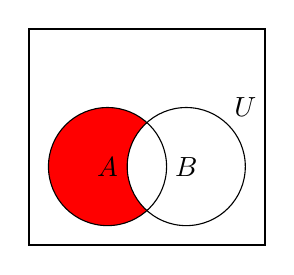
\begin{tikzpicture}[scale=.5]
    
    \def\firstcircle{(0,0) circle (1.5cm)}
    \def\secondcircle{(0:2cm) circle (1.5cm)}
    
    \def\universe{(-2,-2) rectangle (4,3.5)}

    %Color stuff:
    \begin{scope}[even odd rule]
        \clip \secondcircle (0,0) \universe;
        \fill[red] \firstcircle;
    \end{scope}
    
    %draw circles:
    \draw \firstcircle node {$A$};
    \draw \secondcircle node {$B$};
    
    %draw universe:
    \draw[thick] \universe;
    \node at (3.5,1.5) {$U$};
    
    \end{tikzpicture}
    
    bewijs (semi-formeel): \\
    $A-B$: $A$ en $B$ als hierboven; $A-B$ is 3, 6.    
    
    \noindent
    $A-(A\cap B)$: $A\cap B$ is 4, 7; $A-(A\cap B)$ is 3, 6.
    %d:
    \item $A-B=(A\cup B)-B$\\
    antwoord: \\
    Venn diagram:\\
        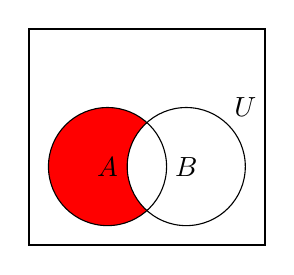
\begin{tikzpicture}[scale=.5]
    
    \def\firstcircle{(0,0) circle (1.5cm)}
    \def\secondcircle{(0:2cm) circle (1.5cm)}
    
    \def\universe{(-2,-2) rectangle (4,3.5)}

    %Color stuff:
    \begin{scope}[even odd rule]
        \clip \secondcircle (0,0) \universe;
        \fill[red] \firstcircle;
    \end{scope}
    
    %draw circles:
    \draw \firstcircle node {$A$};
    \draw \secondcircle node {$B$};
    
    %draw universe:
    \draw[thick] \universe;
    \node at (3.5,1.5) {$U$};
    
    \end{tikzpicture}
    
    bewijs (semi-formeel):\\ 
    $A-B$: als hierboven (3, 6).
    
    \noindent
    $(A\cup B)-B$: $A\cup B$ is 3, 4, 5, 6, 7, 8; $(A\cup B)-B$ is 3, 6.
    % e:
    \item $(A\Delta B)\cap C=(A\cap C)\Delta(B\cap C)$\\
    antwoord:\\
    Venn diagram: \\
    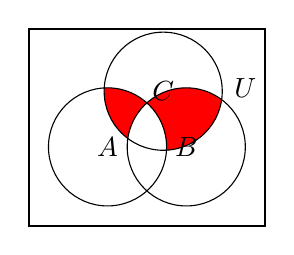
\begin{tikzpicture}[scale=.5]
    
    \def\firstcircle{(0,0) circle (1.5cm)}
    \def\secondcircle{(0:2cm) circle (1.5cm)}
    \def\thirdcircle{(45:2cm) circle (1.5cm)}
    \def\universe{(-2,-2) rectangle (4,3)}

    %Color stuff:
    \begin{scope}[even odd rule]
        \clip \thirdcircle;
        \fill[red] \firstcircle \secondcircle;
    \end{scope}
    %Color more stuff:
    \begin{scope}[even odd rule]
        \clip \thirdcircle;
        \fill[red] \secondcircle\firstcircle;
    \end{scope}
    %color more more stuf:
    % \fill[red] \thirdcircle;
    
    %draw circles:
    \draw \firstcircle node {$A$};
    \draw \secondcircle node {$B$};
    \draw \thirdcircle node {$C$};
    
    
    %draw universe:
    \draw[thick] \universe;
    \node at (3.5,1.5) {$U$};

    \end{tikzpicture}
    
    bewijs (semi-formeel):\\
    $(A\Delta B)\cap C$: $A\Delta B$ is 3, 6, 5, 8; $(A\Delta B)\cap C$ is 3, 5.
    
    \noindent
    $(A\cap C)\Delta(B\cap C)$: $A\cap C$ is 3, 4; $B\cap C$ is 4, 5; $(A\cap C)\Delta(B\cap C)$ is 3, 5.
    
\end{enumerate}
\end{answer}

\begin{answer} % 4.4
Bestudeer de volgende uitspraken. Geef in geval van algemene juistheid een bewijs, geef anders een tegenvoorbeeld.
\begin{enumerate}[label=\textit{\alph*.}]
    \item $A-B=(A\cup C)-(B\cup C)$
    
    Antwoord: Gegeven\\
    \begin{tikzpicture}[scale=.5]
    \def\firstcircle{(0,0) circle (1.5cm)}
    \def\secondcircle{(0:2cm) circle (1.5cm)}
    \def\thirdcircle{(45:2cm) circle (1.5cm)}
    
    \def\universe{(-2,-2) rectangle (4,3.5)}
    
    %draw circles:
    \draw \firstcircle;
    \draw \secondcircle;
    \draw \thirdcircle;
	\node at (-1,-1.25) {$A$};
	\node at (3.25, -1.25) {$B$};
	\node at (0.5, 3) {$C$};   
    
    %draw universe:
    \draw[thick] \universe;
    \node at (3.75,3.25) {$U$};
    \begin{scope}[font=\small, color=hured]
	    \node at (-1, 2) {1};
	    \node at (1.5, 2) {2};
    	\node at (.5,1) {3};
	    \node at (1, .5) {4};
	    \node at (2, 1) {5};
	    \node at (-.5, -.5) {6};
	    \node at (1, -.5) {7};
	    \node at (2.5, -.5) {8};
    \end{scope}
    \end{tikzpicture}\\
    $A$ = 3, 4, 6, 7, $B$ = 4, 5, 7, 8, $C$ = 2, 3, 4, 5.
    
    $A-B$ = 3, 6
    
    $A\cup C$ = 2, 3, 4, 5, 6, 7, $B\cup C$ = 2, 3, 4, 7, 8, $(A\cup C)-(B\cup C)$ = 6.
    
    Tegenvoorbeeld $A=\{1,2\}, B=\varnothing, C=\{2\}$: $A-B=\{1,2\}, (A\cup C)-(B\cup C) = \{1\}$.
    \item $A-B=(A\cap C)-(B\cap C)$
    
    Antwoord: $A-B$ = 3, 6
    
    $A\cap C$ = 3, 4, $B\cap C$ = 4, 5, $(A\cap C)-(B\cap C)$ = 3.
    
    Tegenvoorbeeld $A=\{1,2\}, B=\{3\}, C=\{4\}$, $A-B=\{1,2\}, (A\cap C)-(B\cap C)=\varnothing$.
    \item $(A-B)\cup C=(A\cup C)-(B\cup C)$
    
    Antwoord: $A-B$ = 3,6, $(A-B)\cup C$ = 2, 3, 4, 5, 6.
    
    $A\cup C$ = 2, 3, 4, 5, 6, 7, $B\cup C$ = 2, 3, 4, 5, 7, 8, $(A\cup C)-(B\cup C)$ = 6.
    
    Tegenvoorbeeld $A=\{1,2\}, B=\varnothing, C=\{2\}$: $(A-B)\cup C=\{1,2\}, (A\cup C)-(B\cup C)=\{1\}$.
    \item $(A-B)\cap C=(A\cap C)-(B\cap C)$
    
    Antwoord: $A-B$ = 3, 6, $(A-B)\cap C$ = 3.
    
    $A\cap C$ = 3, 4, $B\cap C$ = 4, 7, $(A\cap C)-(B\cap C)$ = 3.
    
    Stelling is correct.
    \item $(A\Delta B)\cup C=(A\cup C)\Delta(B\cup C)$
    
    Antwoord: $A\Delta B$ = 3, 5, 6, 8, $(A\Delta B)\cup C$ = 2, 3, 4, 5, 6, 8
    
    $(A\cup C)$ = 2, 3, 4, 5, 6, 7, $(B\cup C)$ = 2, 3, 4, 5, 7, 8, $(A\cup C)\Delta(B\cup C)$ = 6, 8.
    
    Tegenvoorbeeld $A=\{1,2,3\}, B=\{2,4,5\}, C=\{1,4,6\}$: $(A\Delta B)\cup C = \{1, 3, 4, 5, 6\}, A \cup C = \{1,2,3,4,6\}, B\cup C = \{1,2,4,5,6\}, (A\cup C)\Delta(B\cup C) = \{ 3, 5\}$.
\end{enumerate}
\end{answer}

\begin{answer} % 4.5
Voor een verzameling $X$ met eindig veel elementen, geven we met $|X|$ het aantal elementen van $X$ aan. Alle in deze opgave voorkomende verzamelingen worden geacht eindig veel elementen te bezitten.
\begin{enumerate}[label=\textit{\alph*.}]
    \item Beredeneer dat $|A\cup B|=|A| + |B| - |A\cap B|$
    
    Antwoord: Ofwel zijn $A$ en $B$ disjoint, dat wil zeggen $A\cap B=\varnothing$, en dan is $|A\cup B|$ gelijk aan alle elementen van $A$ plus die van $B$ ($=|A|+|B|$). 
    
    Ofwel $A$ en $B$ hebben een overlap, dan is $A\cap B\not=\varnothing$; in dat geval zou $|A|+|B|$ de elementen uit $A\cap B$ dubbeltellen (ze zitten immers in $A$ \'en in $B$. Om dit te compenseren moet je dus $|A\cap B|$ van de som van $|A|$ en $|B|$ aftrekken om het juiste aantal elementen in $A\cup B$ te krijgen.
    \item Gebruik het resultaat van a. om aan te tonen dat
    $$|(A\cup B\cup C)=|A|+|B|+|C|-|A\cap B|-|A\cap C|-|B\cap C|+|A\cap B\cap C|.$$
    
%    Antwoord: Aangezien $|A\cup B|=|A|+|B|-|A\cap B|$, kunnen we voor $B$ een andere verzameling naar wens substitueren, bijv. $C\cup D$. We weten dat $|C\cup D|=|C|+|D|-|C\cap D|$, dus 
%    \begin{align*}
%    |A\cup C\cup D| &= |A| + |C\cup D| - |A\cap (C\cup D)|\\
%    &= |A| + |C| + |D| - |C\cap D| - |A\cap (C\cup D)|\\
%    &= |A| + |C| + |D| - |C\cap D| - |(A\cup C)\cap(A\cup D)|
%    \end{align*}
\end{enumerate}
\end{answer}


\begin{answer}\mbox{} % 4.6
\begin{enumerate}[label=\textit{\alph*.}]
\item Gegeven is $A=\{1,2\}$ en $B=\{a,b\}$, bereken $A\times B$;

 Antwoord: $A\times B= \{(1,a), (1,b), (2,a), (2,b)\}$.
\item Gegeven is $A=\{1,2\}$ en $B=\{a,b\}$, bereken $B\times A$;

 Antwoord: $B\times A=\{(a, 1), (a,2), (b,1), (b,2)\}$.
\item Gegeven is $Z=\{0,1,7,8\}$ en $Y=\{0,1\}$, bereken $Z\times Y$;

 Antwoord: $Z\times Y=\{(0,0), (0,1), (1,0), (1,1), (7,0), (7,1), (8,0), (8,1)\}$.
\item Gegeven is $A=\{f,k\}$ en $B=\varnothing$, bereken $A\times B$;

 Antwoord: $A\times B=\varnothing$.
\item Gegeven is $V=\{f,t\}$ en $S=\{c,d,u\}$, bereken $V\times S$.

\noindent Antwoord: $V\times S=\{(f,c), (f,d), (f,u), (t,c), (t,d), (t,u)\}$.
\end{enumerate}
\end{answer}

\begin{answer} % 4.7
Bereken:
\begin{enumerate}[label=\textit{\alph*.}]
\item $\power(A)$ als $A = \{1,3,4,5\}$;

 Antwoord: 
\begin{align*}
\power(A)=\{&\varnothing, \{1\},\{3\},\{4\},\{5\},\\
&\{1,3\},\{1,4\}, \{1,5\}, \{3,4\}, \{3,5\}, \{4,5\},\\
&\{1,3,4\}, \{1,3,5\}, \{1,4,5\}, \{3,4,5\}\\
&\{1,3,4,5\}\}
\end{align*}
\item $\power(B)$ als $B=\{\varnothing, 1,3\}$;

 Antwoord:
\begin{align*}
\power(B)=\{&\varnothing, \{\varnothing\}, \{1\}, \{3\},\\
&\{\varnothing, 1\}, \{\varnothing, 3\}, \{1,3\},\\
&\{\varnothing, 1, 3\}\}
\end{align*}
\item $\power(C)$ als $C=\{1,\{2,3\},\{\{4,5\}\}\}$.

 Antwoord:
\begin{align*}
\power(C)=\{&\varnothing, \{1\}, \{\{2,3\}\}, \{\{\{4,5\}\}\},\\
&\{1,\{2,3\}\}, \{1,\{\{4,5\}\}\}, \{\{2,3\},\{\{4,5\}\}\},\\
&\{1,\{2,3\},\{\{4,5\}\}\}\}
\end{align*}
\end{enumerate}
\end{answer}

\begin{answer}\mbox{} % 4.8
\begin{enumerate}[label=\textit{\alph*.}]
\item Als $A$ een verzameling is en $|A|=5$, wat is dan $|\power(A)|$?

Antwoord: $\power(A)=2^{|A|}=2^5=32$.
\item Als $A$ een verzameling is en $|A|=5$, wat is dan $|A\times A|$?

Antwoord: $|A\times A|=|A|\cdot|A|=5\cdot 5=25$.
\item Als $A=\{12,14,5,1\}$, wat is dan $|(A\times A)\cup A|$?

Antwoord: Omdat $(A\times A)\cap A=\varnothing$ is $|(A\times A)\cup A| = 4\cdot 4 + 4 = 20$.
\end{enumerate}
\end{answer}

\begin{answer} % 4.9
Bepaal voor elk van de volgenden of deze een power set zijn van een of andere verzameling $A$ (en definieer wat $A$ dan precies is). Neem aan dat $a$ en $b$ verschillende elementen zijn.
\begin{enumerate}[label=\textit{\alph*.}]
\item $\varnothing$;

Antwoord: geen powerset.
\item $\{\varnothing,\{a\}\}$;

Antwoord: powerset van $\{a\}$.
\item $\{\varnothing,\{a\},\{\varnothing,\{a\}\}\}$;

Antwoord: geen powerset.
\item $\{\varnothing,\{a\},\{b\},\{a,b\}\}$.

Antwoord: powerset van $\{a,b\}$.
\end{enumerate}
\end{answer}

\begin{answer}[Bonus]\mbox{}\\ % 4.9
Vindt twee verzamelingen $A$ en $B$ zodanig dat $A\in B$ \'en $A\subseteq B$.

\noindent Antwoord: $A=\varnothing$ en $B=\{\varnothing\}$.
\end{answer}

\begin{answer}
  Ga na of de volgende relaties tevens functies zijn:\mbox{}\\
  \begin{enumerate}[label=\textbf{\alph*.}]
    \item de relatie kind-ouder;
    \item de relatie tussen een persoon en de verzameling van diens ouders;
    \item de relatie tussen een persoon en diens vaste partner;
    \item de relatie tussen een geheel getal en het getal met $1$ opgehoogd;
    \item de relatie tussen een getal en het kwadraat van dat getal;
    \item de relatie tussen een getal en de vierkantswortel van dat getal.
  \end{enumerate}
Antwoord:
  \begin{enumerate}[label=\textbf{\alph*.}]
    \item De relatie kind-ouder is geen functie, omdat een kind geen unieke ouder heeft. Ook andersom zou dit niet werken, omdat een ouder ook meerdere kinderen kan hebben.
    \item De relatie tussen een persoon en de verzameling van diens ouders is wel een functie. Ieder kind kan worden afgebeeld op exact een verzameling ouders, waarbij de verzameling uit nul, een of meerdere personen kan bestaan.
    \item De relatie tussen een persoon en diens vaste partner is geen functie, omdat niet iedere persoon een vaste partner hoeft te hebben.
    \item De relatie tussen een geheel getal en het getal met $1$ opgehoogd is een functie, omdat we voor elk (geheel) getal exact een getal kunnen vinden dat $1$ hoger is.
    \item De relatie tussen een getal en het kwadraat van dat getal is een functie: elk getal heeft exact een kwadraat.
    \item De relatie tussen een getal en de vierkantswortel van dat getal is geen functie: voor (bijvoorbeeld) het getal $1$ is er zowel een positieve als negatieve wortel: $-1$ en $1$.
  \end{enumerate}

\end{answer}

\begin{answer}\mbox{}\\
  \begin{enumerate}[label=\textbf{\alph*.}]
    \item Gegeven zijn de verzamelingen $K = \{ \text{Wilhelmina}, \text{Juliana}, \text{Beatrix},$\\ $\text{Willem-Alexander}, \text{Amalia} \}$ en de volgende pijlen:
  \begin{align*}
    \text{Wilhelmina} &\longrightarrow \text{Juliana}\\
    \text{Juliana} &\longrightarrow \text{Beatrix}\\
    \text{Beatrix} &\longrightarrow \text{Willem-Alexander}\\
    \text{Willem-Alexander} &\longrightarrow \text{Amalia}
  \end{align*} Hebben we hier met een geldige functie $K \to K$ te maken?\\ Zo nee, wat zouden we moeten aanpassen om wel een geldige functie te defini\"{e}ren?\\

  \item Gegeven zijn de verzameling $H = \{ \text{steen}, \text{papier}, \text{schaar} \}$ en de volgende pijlen:
  \begin{align*}
    \text{steen} &\longrightarrow \text{schaar}\\
    \text{papier} &\longrightarrow \text{steen}\\
    \text{schaar} &\longrightarrow \text{papier}
  \end{align*} Hebben we hier met een geldige functie $H \to H$ te maken?\\ Zo nee, wat zouden we moeten aanpassen om wel een geldige functie te defini\"{e}ren?
  \end{enumerate}
  Antwoord:
  \begin{enumerate}[label=\textbf{\alph*.}]
    \item Nee, in dit voorbeeld is er geen pijl die vertrekt vanuit Amalia. Hier zouden we een bestaand element in de set voor moeten vinden --- zo niet dan verschuiven we het probleem naar het nieuwe element omdat daar dan ook nog geen pijl uit vertrekt.
    Als we de betekenis van de kandidaat-functie interpreteren als \enquote{$x$ heeft als kind $y$} dan zien we dat het lastig zal worden een verzameling te vinden waar voor ieder persoon een kind te vinden is, omdat we dan een cyclus of oneindige verzameling nodig hebben. Helaas gaat ouderschap (biologisch gezien) niet in cirkels, dus deze oplossing vervalt binnen deze semantische context. Een betere oplossing zou zijn om het domein en codomein los van elkaar t ehalen. Het domein zou nu een deelverzameling zonder Amalia zijn, het codomein moet Amalia juist wel bevatten.
    \item Ja, in dit voorbeeld kunnen we voor elke waarde in het domein een waarde in het codomein aanwijzen. In tegenstelling tot de vorige vraag hebben we hier wel een cyclus.
  \end{enumerate}

\end{answer}

\begin{answer}\mbox{}\\
  \begin{enumerate}[label=\textbf{\alph*.}]
    \item Gegeven zijn de verzameling $S = \{ \text{winter}, \text{lente}, \text{zomer}, \text{herfst} \}$ en de afbeelding $v : S \to S$:
  \begin{equation*}
  \begin{aligned}
    \text{winter} &\longrightarrow \text{lente}\quad\quad\quad &
    \text{zomer} &\longrightarrow \text{herfst}\\
    \text{lente} &\longrightarrow \text{zomer}&
    \text{herfst} &\longrightarrow \text{winter}
  \end{aligned}
  \end{equation*}
  \begin{enumerate}[label=\textbf{\alph*.}]
      \item Wat is de waarde van $v(\text{zomer})$?
      \item Wat is het type\footnote{Tot welke verzameling behoort deze waarde?} van $v(\text{zomer})$?
      \item Heeft het zin om over de waarde $v(v(\text{winter}))$ te redeneren?\\ Zo ja: wat is deze waarde; zo nee: waarom niet?\\
  \end{enumerate}

  \item Gegeven zijn de verzamelingen $D_{1} = \{ \text{David}, \text{Matt}, \text{Peter} \}$, $D_{2} = \{ \text{Matt}, \text{Peter}, \text{Jodie} \}$ en de afbeelding $r : D_{1} \to D_{2}$:
  \begin{equation*}
  \begin{aligned}
    \text{David} &\longrightarrow \text{Matt}\quad\quad
    \text{Peter} &\longrightarrow \text{Jodie}\\
    \text{Matt} &\longrightarrow \text{Peter}
  \end{aligned}
  \end{equation*}
  \begin{enumerate}[label=\textbf{\alph*.}]
      \item Wat is de waarde van $r(\text{David})$?
      \item Wat is het type van $r(\text{David})$?
      \item Heeft het zin om voor $x \in D_{1}$ over de waarde $r(r(x))$ te redeneren?\\ Beargumenteer je antwoord.
  \end{enumerate}
  \end{enumerate}
Antwoorden:
  \begin{enumerate}[label=\textbf{\alph*.}]
    \item \begin{enumerate}[label=\textbf{\alph*.}]
             \item herfst
             \item $S$
             \item Ja: de waarde $v(\text{winter})$ zit in het domein van $v$, waardoor we $v$ hier dus op kunnen aanroepen om te vinden dat $v(v(\text{winter})) = zomer$
          \end{enumerate}
    \item \begin{enumerate}[label=\textbf{\alph*.}]
             \item Matt
             \item $D_{2}$
             \item Nee: de waarde $r(\text{x}) \in D_{2}$ zit niet in het domein $D_{1}$ van $r$, waardoor we $r$ hier niet zomaar op kunnen aanroepen. In het geval dat $r(x)$ in beide verzamelingen zit dan is het mogelijk $r(r(x))$ te vinden, maar in het algemeen is dit niet mogelijk. Neem als tegenvoorbeeld $x = \text{Peter}$ zodat $r(x) = \text{Jodie} \not\in D_{1}$.
          \end{enumerate}
  \end{enumerate}
\end{answer}

\begin{answer}\mbox{}\\
  \begin{enumerate}[label=\textbf{\alph*.}]
    \item Gegeven is de functie $f(x) = 2x + 1$. We kunnen hier verschillende keuzes voor het domein maken; het codomein zal hiervan afhankelijk zijn.
      \begin{enumerate}
        \item Wat is het codomein als het domein $\mathbb{N}$ is?
        \item Wat is het beeld\footnote{Hint: voor deze verzameling hebben we geen symbool zoals $\mathbb{N}$, maar toch is deze eenduidig te beschrijven als deelverzameling van het codomein dat je al gevonden hebt.} als het domein $\mathbb{N}$ is?
        \item Wat is het codomein als het domein $\mathbb{R}$ is?
      \end{enumerate}

    \item Gegeven is de functie $f(x) = 3^{x} - 2$. We kunnen hier verschillende keuzes voor het domein maken; het codomein zal hiervan afhankelijk zijn.
      \begin{enumerate}
        \item Wat is het codomein als het domein $\mathbb{N}$ is?
        \item Wat is het codomein als het domein $\mathbb{N}_{1}$ is, waarbij $\mathbb{N}_{1} = \mathbb{N} - \{0\}$, oftewel de verzameling van alle positieve gehele getallen?
        \item Wat is het codomein als het domein $\mathbb{Z}$ is?
        \item Wat is het codomein als het domein $\mathbb{Q}$ is?
      \end{enumerate}


  \end{enumerate}

  Antwoorden:

  \begin{enumerate}[label=\textbf{\alph*.}]
    \item \begin{enumerate}
        \item Het getal $x$ is een natuurlijk getal; als we een natuurlijk getal verdubbelen dan blijft dit een natuurlijk getal, en ook met het $1$ erbij optellen blijven we in $\mathbb{N}$.
        \item Voor de eerste natuurlijke getallen $(0,1,2,3,\dots)$ komen we op de waardes $(1,3,5,7,\dots)$. Dit zijn de oneven natuurlijke getallen.
        \item Het getal $x$ is nu een re\"{e}el getal. Door dit te verdubbelen of er $1$ bij op te tellen zal hier niets aan veranderen: het getal wordt niet ineens rationeel als het dat niet al was, en blijft dus in $\mathbb{R}$. \emph{Extra: hoewel we deze cursus geen getalverzamelingen groter dan $\mathbb{R}$ beschouwen is het in dit geval ook niet zo dat we een groter getalsysteem nodig zouden hebben. Voor complexe getallen moet de wortel van een negatief getal genomen worden, wat hier niet gebeurt.}
      \end{enumerate}


    \item \begin{enumerate}
        \item Voor een natuurlijke $x$ wordt $3^{x}$ een natuurlijk getal in de verzameling $\{ 1, 3, 9, 27, \dots \}$. Als we hier hier $2$ van aftrekken dan komen we uit op een getal uit de verzameling $\{ -1, 1, 7, 25, \dots \}$. $-1$ is geen natuurlijk getal maar een integer, de andere getallen zijn allemaal natuurlijke getallen en daarmee ook integers. Het codomein is dus $\mathbb{Z}$.
        \item Voor een gehele positieve $x$ is het scenario hetzelfde als hierboven, behalve dat de eerste waarde $-1$ niet in het beeld van de functie zit. De mogelijke waardes zijn hiermee beperkt tot de natuurlijke getallen $\mathbb{N}$.

        \item Voor een gehele $x$ blijft het bovenstaande scenario bestaan, maar kunnen we ook een negatief exponent bij $3^{x}$ krijgen. Negatieve exponenten staan gelijk aan breuken, zo dat $x^{-n} = \frac{1}{x^{n}}$. Het aftrekken van $2$ van een breuk zal opnieuw een breuk opleveren, dus we zitten hier in de rationele getallen $\mathbb{Q}$.
        \item Voor een rationele $x$ kunnen we ook breuken in het exponent verwachten, zoals $3^{\frac{1}{2}}$. Dit staat gelijk aan $\sqrt{3}$, een irrationeel getal. Het codomein van de functie moet daarmee tenminste $\mathbb{R}$ zijn. \emph{Extra: dit is de grootste verzameling getallen die we voor deze cursus beschouwen, maar ook in dit geval hebben we geen complexe getallen nodig. Hoewel het met rationele exponenten mogelijk is wortels te trekken, zal deze wortel altijd van het positieve getal $3$ genomen worden en blijven we dus op de re\"{e}le getallenlijn.}
      \end{enumerate}

  \end{enumerate}
\end{answer}
